\chapter{Nonverbal Immediacy for use with Children and Robots} \label{chap:validation}

\begin{framed}
	\textbf{Key points:}
	
	\begin{itemize}
	\item Nonverbal immediacy has been used extensively in adult lecture scenarios, where higher \gls{nonverbalimm} is correlated with increased learning.
	\item Three different characters were used to read a story to both children and adults: an intended high \gls{nonverbalimm} robot, low \gls{nonverbalimm} robot, and a human.
	\item Both adults and children perceived the robot conditions as intended with respect to \gls{nonverbalimm}. Adults and children also rate the behaviour of all three characters in a similar manner.
	\item Children recall more of the story from the robot with high \gls{nonverbalimm}.
	\item These findings confirm hypotheses generated from the \gls{nonverbalimm} literature, and provide a link between child-robot interaction and this literature.
	\end{itemize}
\end{framed}

Part of the work presented in this chapter has been published in \cite{kennedy2016nonverbal}. The final publication is available from Springer via: \newline http://dx.doi.org/10.1007/s12369-016-0378-3

\newpage
Nonverbal immediacy has been used extensively in adult human studies, often in lecture scenarios \citep{christophel1990relationships, gorham1988relationship, thweatt1998impact}. It has also seen limited application in \acrshort{hri} evaluations (Chapter~\ref{chap:background}), and where this has been done, the \gls{immediacy} scores have not been explicitly stated. As such, it is desirable to validate that behavioural manipulations of \gls{nonverbalimm} when applied to a robot are perceived and reported as intended. Additional validation with children to check whether they interpret the behaviour in the same manner as adults would provide a solid basis for proceeding with using \gls{nonverbalimm} in child-robot tutoring scenarios. This also provides a further link between the adult human \gls{immediacy} literature and child-robot interactions, which can be useful in hypothesis generation and discussion of results. This chapter presents a study which aims to bridge the gap between the adult human literature and the child-robot interactions under consideration in this thesis. In particular, the study seeks to explore whether the \gls{nonverbalimm} measure can be understood by children, whether children perceive manipulations in \gls{nonverbalimm}, and whether the positive correlation between \gls{nonverbalimm} and recall observed with adults also applies to children. If successful, this could then be used as a means of characterising robot social behaviour, and also assist in designing the robot behaviour (given the explicit list of cues that form the NVI metric).

%%%%%%%%%%%%%%%%%%%%%%%%%%%%%%%%%%%%%%%%%%%%%%%%%%%%%%%%%%%%%%%%%%%%%%%
\section{Hypotheses}
Based on the literature explored in Chapter~\ref{chap:background}, three hypotheses for the study were devised, in addition to a manipulation check. Chapter~\ref{chap:background} explored the \gls{nonverbalimm} literature, finding that several researchers have found a link between increased perceptions of \gls{nonverbalimm} and learning or recall \citep{comstock1995food,mccroskey1996nonverbal,witt2004meta}. This has also been found for some robot behaviours when evaluated with adults \citep{szafir2012pay}. These findings lead to a consideration of whether this effect will also be observed with children. To provide a greater link between the adult literature and the child-focussed group under consideration in this thesis, both the effect on perceptions of \gls{nonverbalimm} and recall will be considered, leading to hypotheses H1 and H2. The effect at the group level will be explored through these hypotheses, with a further hypothesis devised to consider the impact of \gls{nonverbalimm} perception on recall at the individual level in H3. The outcome here will demonstrate whether changes in \gls{nonverbalimm} behaviours are perceived by children, and whether the link between NVI and learning from the \gls{nonverbalimm} literature applies when interacting with robots.
\begin{itemize}
	\item [\textbf{H1}:] Recall of a story will be greater when read by a character with higher \gls{nonverbalimm}.
	\item [\textbf{H2}:] Children and adults will perceive \gls{nonverbalimm} in the same manner for both robots and humans (i.e., children and adults ranking of immediacy will agree).
	\item [\textbf{H3}:] As \gls{nonverbalimm} of the character reading a story is perceived to increase by an individual, their recall of the story will also increase.
\end{itemize}

As the robot behaviour is intentionally manipulated along the nonverbal immediacy measure (further details in Section~\ref{sec:ch4-conditions}), a manipulation check was conducted to verify that robot behaviour designed to be more or less immediate is perceived as such, as measured through the \gls{nonverbalimm} scale.

%%%%%%%%%%%%%%%%%%%%%%%%%%%%%%%%%%%%%%%%%%%%%%%%%%%%%%%%%%%%%%%%%%%%%%%
\section{Experimental Setup} \label{sec:nvi-setup}
A 2 (adults vs. children) x 3 (high NVI robot, low NVI robot, human) between-subject study was devised to explore how \gls{nonverbalimm} would impact recall and to evaluate whether children and adults interpret the behaviour of a robot and a human in the same way. In order to achieve this, a scenario which could be understood by both groups was required. As such, the study design started from the perspective of the children (who are presumed to have a shorter attention span and more limited knowledge in some areas such as vocabulary) and was then applied to adults. Recall of a presented short story was decided to be an appropriate task for this purpose as this matched the lecture-style scenarios of \gls{immediacy} studies \citep{gorham1988relationship, thweatt1998impact}.

\begin{figure}[t!]
    \centering
    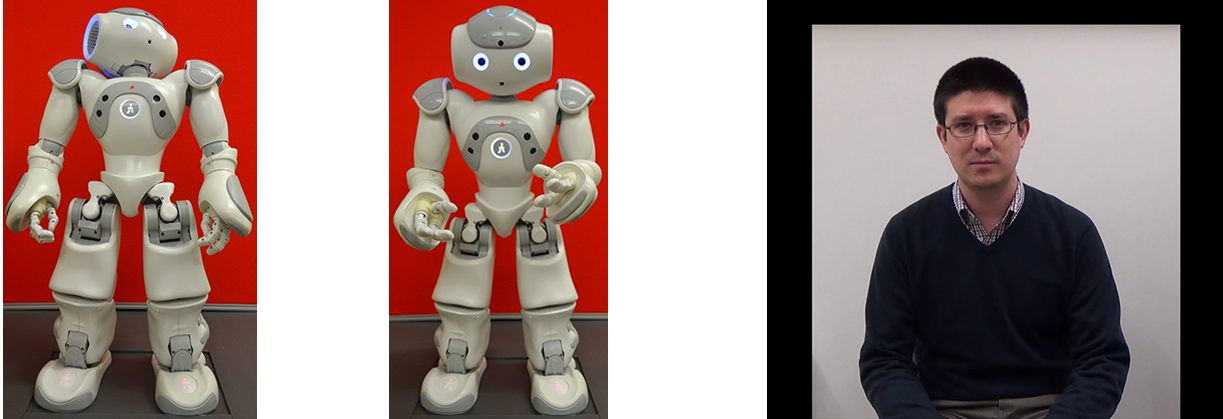
\includegraphics[width=0.9\textwidth]{images/ch4_conditions.png}
    \caption{Still images from the conditions used in the evaluation; \textit{left} to \textit{right}: (1) low nonverbal immediacy robot, (2) high nonverbal immediacy robot, (3) human. Red backgrounds for the robot were not used in practice and are just used to ease visibility here; the video was shown in widescreen format, with a black background covering the unused space, as in the figure.}
    \label{fig:ch4_conditions}
\end{figure}

\subsection{Participants}
A total of 117 participants took part in the study, but one child had to be excluded due to an incomplete questionnaire and two adults were excluded due to inconsistent online video timestamps; this will be expanded on later in this section. 83 children (age \textit{M}=7.8 years, \textit{SD}=0.7; 47 F, 36 M) and 31 adults (age \textit{M}=23.5 years, \textit{SD}=3.9; 7 F, 24 M) remained for data analysis. All participants consented to participation in the study and all children had parental permission to take part. The children were recruited from one school year group of a primary school in the U.K.; the children were split across conditions based on their usual school classes, which ensures an appropriate balance for gender and academic ability. Adults in the robot conditions were recruited through regular lectures, and through online advertising for the human condition.

\subsection{Short Story}
A short story was created for the purpose of the recall test. The story was largely based on one freely available from a website containing many short stories for children\footnote{\href{http://freestoriesforkids.com/children/stories-and-tales/robot-virus}{http://freestoriesforkids.com/children/stories-and-tales/robot-virus}}. This was done to make sure that the language and content was appropriate for children. Some elements were added or modified in order to create opportunities for recall questions, and some of the phrasing was modified so that the robot text-to-speech sounded more accurate. The final version of the story created can be seen in Appendix~\ref{app:story_questions} and lasts for just under four minutes when read in the experimental conditions. None of the participants reported to have heard or read the story before.

\subsection{Measures} \label{sec:ch4-measures}
Two measures were used: a \gls{nonverbalimm} observer report questionnaire and a recall test. The \gls{nonverbalimm} questionnaire is described in Chapter~\ref{chap:method} and can be seen in Appendix~\ref{app:rniq}. The recall test was devised based on information provided in the short story and consisted of 10 multiple choice questions, with a final free text answer about the moral of the story. The full list of questions and answer options can be seen in Appendix~\ref{app:story_questions}. The questions were designed to vary in difficulty based on how many times the piece of information had been stated, how central it was to the plot, and how many answer options were similar to the correct one. An additional question was added to the adult human condition regarding the colour of the background in the video; this was part of a series of checks to ensure that the video had actually been watched.

\subsection{Conditions} \label{sec:ch4-conditions}
In order to address the hypotheses for the study, three conditions were devised which were shown to both children and adults. Two conditions use a robot that has the social behaviour manipulated along the \gls{nonverbalimm} scale, while the third uses a human to provide a control condition, given the novelty of applying \gls{nonverbalimm} to robot social behaviour.
\begin{enumerate}
	\item \textbf{High \gls{nonverbalimm} robot} (Fig.~\ref{fig:ch4_conditions} \textit{centre}) - the robot behaviour was maximised for immediacy where possible; full details of the robot behaviour can be seen in the following paragraph. Child \textit{n}=27; adult \textit{n}=9.
	\item \textbf{Low \gls{nonverbalimm} robot} (Fig.~\ref{fig:ch4_conditions} \textit{left}) - the robot behaviour was minimised for immediacy where possible; full details of the robot behaviour can be seen in the following paragraph. Child \textit{n}=28; adult \textit{n}=9.
	\item \textbf{Human} (Fig~\ref{fig:ch4_conditions} \textit{right}) - a human was recorded on video reading the story to provide a control condition. Video was used to ensure identical behaviour between child and adult groups and to time the story to be at the same pace as the robot conditions in order to have equivalent exposure time and reading speeds (which can impact recall; \citealp{hulme1989working, simonds2006effects}). The human was not given explicit instructions in terms of nonverbal behaviour, as their \gls{immediacy} level is not under consideration, but whether the children and adults perceive their immediacy level in the same way is. Therefore, the behaviour itself is not of concern, provided that it is identical between conditions. Child \textit{n}=28; adult \textit{n}=13.
\end{enumerate}

\afterpage{%
	\begin{landscape}
		\begin{table}[t!]
		\centering
		\renewcommand{\arraystretch}{1.2} 
		\begin{tabular}{@{}>{\raggedright}p{3cm}p{9.25cm}p{9.25cm}@{}}
		\toprule
		\textbf{Behavioural Dimension} & \textbf{High Nonverbal Immediacy} & \textbf{Low Nonverbal Immediacy} \\ \midrule
		Gesture				& Frequent gestures, occurring approximately every 12 seconds during the story. Slight randomness added to joints to provide small constant movement.		& No gestures, no joint random movement.                        \\
		Gaze					& Head gaze directed forwards randomly at approximately the same height as the robot towards the centre of the movement range (towards observers).		& Head gaze directed randomly up and towards the corners of movement range (over/away from observers).                       \\
		Vocal prosody	& No modifications to standard text-to-speech (TTS) engine, allowing shaping of sentences and responsiveness to punctuation.			& All strings passed to TTS have punctuation stripped and are forced to be spoken with no context of the sentence (resulting in words sounding identical every time they are said). Additionally, vocal shaping was reduced via a TTS parameter.                        \\
		Body orientation		& Leans towards observers by approximately 15 degrees.	 & Leans away from observers by approximately 15 degrees.                        \\ \bottomrule
		\end{tabular}
		\caption{Operationalisation of behavioural manipulations between robot immediacy conditions}
		\label{table:ch4_behave}
		\end{table}
	\end{landscape}
}

\subsection{Robot Behaviour}
The high and low \gls{nonverbalimm} robot conditions were developed by maximising and minimising dimensions of the \gls{nonverbalimm} scale, as described in Chapter~\ref{chap:method}. The conditions sought to maximise the differences between the behavioural dimensions and therefore also the dimensions measured by the \gls{nonverbalimm} scale. Some dimensions were not varied due to limitations in the experimental set-up. Facial expressions were not varied as the robot being used for the study, an Aldebaran NAO, is not capable of producing facial expressions such as frowning or smiling. Proximity was not varied due to the group setting in which the study was being conducted. When the robot is telling the story to a classroom of children it is not feasible, or safe, to incorporate touch or to approach the children. The operationalisation of behavioural manipulations that were carried out can be seen in Table~\ref{table:ch4_behave}.

\subsection{Procedure}
For the robot conditions, the robot was placed at the front of the classroom on a table to be roughly at the head height of observers (either children or adults). The experimenter would then explain that the robot would read a story and that afterwards they would be required to fill in a questionnaire about what they thought of the robot. The recall test was explicitly not mentioned to prevent participants from actively trying to memorise the story. The experimenter then pressed a button on the robot's head to start the story. Once the story was complete, the \gls{nonverbalimm} questionnaires were provided to all participants. When the whole group had completed this questionnaire, the recall test was introduced and given to participants. For the children, this was followed by a short demonstration of the robot. The human video condition procedure was the same for the children. The video was resized to match the size of the robot as closely as possible, and the volume was adjusted to be approximately the same as well.

As the children did not know this person, the adults should not either so that the reported \gls{immediacy} score is based purely on the behaviour seen in the video and not prior interaction. The subjects for the video condition were recruited online and completed a custom web form which prevented the video from being paused or played more than once, and recorded timestamps for the start of the video, the end of the video, and the completion of the questions. An additional question about the background of the video was also added to the recall test to verify that the participants had actually watched the video (as opposed to the rest of the recall questions which can be answered through listening alone; described in Section~\ref{sec:ch4-measures}). One participant was excluded from analysis as the timestamps for the start and end of the video indicated too little time for the full video to have been viewed and another participant was excluded as the time between watching the video and completing the questions was in the order of hours (all other participants completed all questions in under 10 minutes), indicating that the intended protocol had been violated.

%%%%%%%%%%%%%%%%%%%%%%%%%%%%%%%%%%%%%%%%%%%%%%%%%%%%%%%%%%%%%%%%%%%%%%%
\section{Results} \label{sec:nvi-results}
\subsection{Nonverbal Immediacy Results} \label{sec:res-imm}
Cronbach's alpha values were calculated for the \gls{nonverbalimm} questionnaire for adults and children, splitting the human condition and the robot conditions. All alpha values are based on the 16 item scale. The reliability rating for the adults with the robot is high ($\alpha=.79$), whereas in the human condition it is quite a bit lower ($\alpha=.45$). This difference may be an effect of embodiment, and will be explored further in the discussion Section~\ref{sec:disc-nvi}. Reliability scores for children are relatively low in both cases (human $\alpha=.55$; robot $\alpha=.30$). The implications of this are also discussed in Section~\ref{sec:disc-nvi}.

Nonverbal immediacy scores were calculated from the questionnaires and produce a number which can be between 16 and 80. Immediacy scores and confidence intervals can be seen for each condition in Table~\ref{table:ch4_immediacy}. Whilst these scores might initially appear to be relatively low given the possibility of scores as high as 80, the scores do fall in the range expected. Due to the exclusion of certain aspects of the \gls{immediacy} inventory in the robot conditions in terms of moving towards and touching observers, as well as producing facial expressions, it is unlikely that the score would raise above 56. It is however possible to be perceived differently and score more highly (for example the robot could have been perceived to have produced a smile, even though the mouth cannot move).

For the robot conditions, two groups were used with independence of observations, and a continuous measure for nonverbal immediacy. Distributions did not significantly deviate from normality (Kolmogorov-Smirnov test; $\textit{p}>.05$) and had homogeneity of variances (Levene's test; $\textit{p}>.05$). For this reason, two-tailed independent samples \textit{t}-tests are used to analyse the results for both children and adults. A two-tailed \textit{t}-test on the adult data reveals a significant difference between the \gls{nonverbalimm} score for the high immediacy robot (\textit{M}=50.2, 95\% CI [47.0,53.5]) and the low immediacy robot (\textit{M}=36.3, 95\% CI [33.5,39.1]); \textit{t}(16)=7.460, \textit{p}\textless .001. The same test on the child data also reveals a significant difference between the \gls{nonverbalimm} score for the high immediacy robot (\textit{M}=50.8, 95\% CI [48.6,53.0]) and the low immediacy robot (\textit{M}=46.5, 95\% CI [44.2,48.8]); \textit{t}(53)=2.793, \textit{p}=.007 (Figure~\ref{fig:ch4_immgraph}). These results confirm that the manipulation was successful: the robot behaviour designed to be more or less immediate is perceived as such when measured using the \gls{nonverbalimm} scale. This provides a useful check that the behaviour of the robot has been interpreted as intended by both children and adults.

Support can be seen for hypothesis H2, that children and adults will perceive \gls{nonverbalimm} in the same manner for both robots and humans (Table~\ref{table:ch4_immediacy}). The results show that both children and adults score the high immediacy robot very similarly, with almost identical means. The relative ranking of \gls{immediacy} between conditions is also the same, with the high immediacy robot being perceived as most immediate, then the human, followed by the low immediacy robot condition. 

However, there are also some differences as the child scores are more tightly bunched together; this could reflect their different (yet consistent) interpretation of negatively formulated questions \citep{borgers2004response}, or more limited language understanding impeding the data quality \citep{borgers2000children}. A two-way ANOVA was conducted to examine the effect of age group (child/adult) and condition (high/low robot, human) on the \gls{immediacy} rating. These groups were used with two independent variables, independence of observations between groups, and a continuous measure. Distributions did not significantly deviate from normality (Kolmogorov-Smirnov test; $\textit{p}>.05$) and had homogeneity of variances (Levene's test; $\textit{p}>.05$). A significant interaction effect was found between age group and condition: \textit{F}(2,108)=5.29, \textit{p}=.006. Whilst both age groups rated the human to have lower NVI than the high immediacy robot, and the low immediacy robot in turn lower than the human, this difference was more pronounced for the adult age group. Significant main effects were found for condition (\textit{F}(2,108)=16.96, \textit{p}$<$.001) and age (\textit{F}(1,108)=26.51, \textit{p}$<$.001). However, due to the interaction effect between age group and condition, exploration of simple main effects splitting the conditions is also required to correctly interpret the results. Significant simple main effects are found for condition within each level of age group (child/adult): adults -- Wilks' Lambda=.796, \textit{F}(4,214)=6.46, \textit{p}$<$.001; children -- Wilks' Lambda=.798, \textit{F}(4,214)=6.38, \textit{p}$<$.001. Significant simple main effects are also found for age group within each condition: low immediacy robot -- Wilks' Lambda=.664, \textit{F}(2,107)=27.11, \textit{p}$<$.001; high immediacy robot -- Wilks' Lambda=.862, \textit{F}(2,107)=8.54, \textit{p}$<$.001; human --Wilks' Lambda=.811, \textit{F}(2,107)=12.49, \textit{p}$<$.001.

These findings suggest that some differences are present in the way that children perceive (or at least report) the \gls{immediacy} of the characters when compared to adults. This is not surprising given the tighter bunching of child \gls{nonverbalimm} scores. Nevertheless, there is a strong positive correlation between the child scores and the adult scores, \textit{r}(1)=0.91, although this is not significant (\textit{p}=.272) due to the low number of comparisons (3 conditions). Overall, due to the strong positive correlation and the same ranking of the conditions, it would seem that children perceive \gls{nonverbalimm} in a similar manner as adults, but there are clearly some differences at least in terms of reporting. We would argue that there is a strong enough link to deem \gls{nonverbalimm} an appropriate measure to use with children (and to tie the findings here to the adult human immediacy literature), but this is an area that would benefit from further research.

\begin{table}[t!]
	\centering
	\renewcommand{\arraystretch}{1.2} 
	\begin{tabular}{@{}lllll@{}}
	\toprule
	\textbf{Condition}			& \textbf{Adult \textit{M}}	& \textbf{95\% CI}	& \textbf{Child \textit{M}} 	& \textbf{95\% CI}	\\ \midrule
	High immediacy robot	& 50.2           				& [47.0,53.5]	& 50.8					& [48.6,53.0]		\\
	Low immediacy robot 	& 36.3 						& [33.5,39.1]	& 46.5					& [44.2,48.8]		\\
	Human								& 41.5						& [38.4,44.5]	& 49.7					& [47.0,52.4]		\\ \bottomrule
	\end{tabular}
	\caption{Mean nonverbal immediacy scores by condition}
	\label{table:ch4_immediacy}
\end{table}

\begin{figure}[t!]
	\centering
    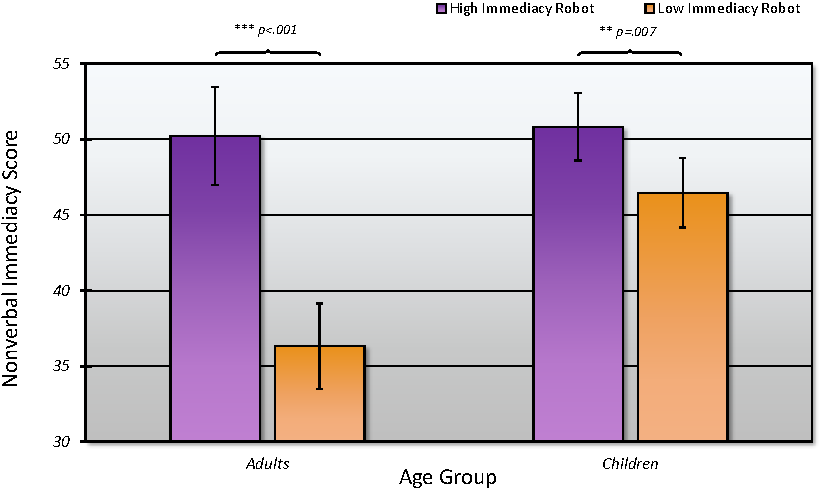
\includegraphics[width=0.8\textwidth]{images/ch4_RobotImmGraph.pdf} \\
   \caption{Robot nonverbal immediacy scores as rated by children and adults, relating to hypothesis H2. Both children and adults perceive the difference in nonverbal immediacy between the two robot conditions. ** indicates significance at the \textit{p}\textless .01 level, and *** indiciates significance at the \textit{p}\textless .001 level. \textit{Error bars} show the 95\% Confidence Interval}
    \label{fig:ch4_immgraph}
\end{figure}

%%%%%%%%%%%%%%%%%%%%%%%%%%%%%%%%%%%%%%%%%%%%%%%%%%%%%%%%%%%%%%%%%%%%%%%
\subsection{Recall Results} \label{sec:res-recall}
Recall results are based on the 10 recall questions presented to all participants; scores are given as the correct proportion of answers, i.e., 8 correct answers = 0.8. Recall scores and confidence intervals can be seen for each condition in Table~\ref{table:ch4_recall} and are represented graphically in Figure~\ref{fig:ch4_recallgraph}.

To explore hypothesis H1, a comparison in recall was made on the adult data between those observing the high and low immediacy robot conditions. Two groups were used with independence of observations, and a continuous measure. Distributions did not significantly deviate from normality (Kolmogorov-Smirnov test; $\textit{p}>.05$) and had homogeneity of variances (Levene's test; $\textit{p}>.05$). For this reason, two-tailed independent samples \textit{t}-tests are used to analyse the results. No significant differences at the \textit{p}\textless .05 level were found; \textit{t}(16)=-0.577, \textit{p}=.572. However, significant differences are found for the child data. A two-tailed independent samples \textit{t}-test reveals that recall is higher in the high immediacy robot condition (\textit{M}=0.58, 95\% CI [0.52,0.64]) than in the low immediacy robot condition (\textit{M}=0.49, 95\% CI [0.46,0.53]); \textit{t}(53)=2.006, \textit{p}=.011.

These results provide partial support for hypothesis H1: recall will be greater when the character reading the story is more nonverbally immediate. It can be seen that this holds true for the children, where recall is greater in the high immediacy robot condition than in the low immediacy robot condition, in accordance with this condition being perceived as more immediate. However, there are no significant differences in recall between the conditions for adults. This is likely due to a ceiling effect with adults because the recall questions were designed so that they were suitable for children. This may have made them too easy for adults overall, leaving limited space to show differences between conditions. If the questions were more difficult and exclusively targeted towards adults then it is possible that differences would be found. The partial support for H1 and replication of findings from previous studies of \gls{nonverbalimm} -- using robots -- provides a proof-of-concept for the approach.

No support is found for hypothesis H3: that higher individual perception of \gls{nonverbalimm} will lead to greater recall for that individual. Correlations between \gls{nonverbalimm} ratings and recall scores are not significant for children (\textit{r}(81)=-0.047; \textit{p}=.673) or adults (\textit{r}(29)=-0.188; \textit{p}=.311). Indeed the correlations themselves are in the opposite direction (although only with a small magnitude) to that which was expected. This would suggest that in this study, the rating of immediacy at the individual level has less of a bearing on recall than the average as judged by the group, but there is not enough evidence here to explain why this occurred.

\begin{table}[t!]
	\centering
	\renewcommand{\arraystretch}{1.2} 
	\begin{tabular}{@{}lllll@{}}
	\toprule
	\textbf{Condition}		& \textbf{Adult \textit{M}}	& \textbf{95\% CI}	& \textbf{Child \textit{M}} & \textbf{95\% CI}			\\ \midrule
	High immediacy robot	& 0.80      & [0.69,0.91]	& 0.58		& [0.52,0.64]		\\
	Low immediacy robot 	& 0.83 		& [0.76,0.91]	& 0.49		& [0.46,0.53]		\\
	Human					& 0.79		& [0.73,0.84]	& 0.63		& [0.56,0.70]		\\ \bottomrule
	\end{tabular}
	\caption{Mean recall scores by condition}
	\label{table:ch4_recall}
\end{table}

\begin{figure}[t!]
\centering
    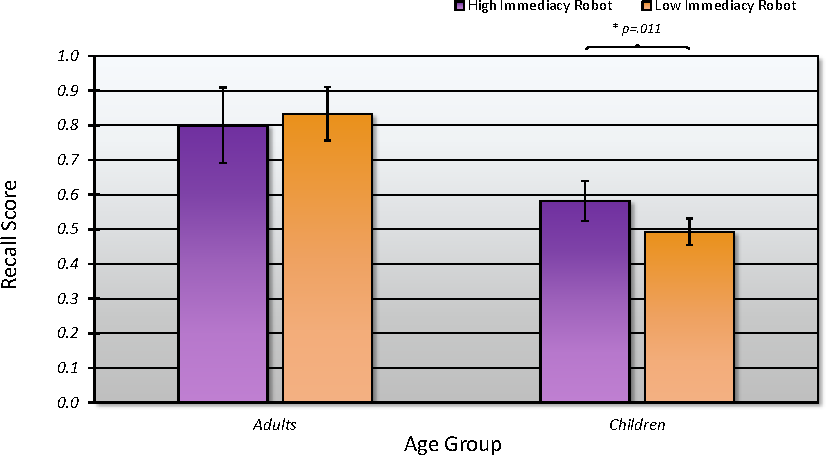
\includegraphics[width=0.8\textwidth]{images/ch4_RecallGraph.pdf} \\
   \caption{Recall scores for high and low nonverbal immediacy robot conditions relating to hypothesis H1. Children recall significantly more information when the story is read by a robot with higher nonverbal immediacy. * indicates significance at the \textit{p}\textless .05 level. \textit{Error bars} show the 95\% Confidence Interval}
    \label{fig:ch4_recallgraph}
\end{figure}

%%%%%%%%%%%%%%%%%%%%%%%%%%%%%%%%%%%%%%%%%%%%%%%%%%%%%%%%%%%%%%%%%%%%%%%
\section{Discussion} \label{sec:nvi-discussion}
The established research field of \textit{\gls{nonverbalimm}} links behaviour to learning gains in a measurable and comparable manner (Chapter~\ref{chap:background}). The evaluation in this chapter applied behaviour based on \gls{nonverbalimm} cues to a social robot. It was found that both children and adults perceive the immediacy of a robot designed to have low and high \gls{nonverbalimm} behaviours as intended, which confirms and extends prior work in \acrshort{hri} \citep{szafir2012pay}. Additionally, both children and adults ranked the \gls{nonverbalimm} of robots and humans in the same order, although children's raw scores were more tightly grouped. This gives rise to the possibility that much of the \gls{nonverbalimm} literature, which has mostly been conducted with adults, would also apply to children.

Recall of a short story improved significantly for children when the robot reading the story was more immediate in behaviour, which does indeed confirm the hypothesis derived from nonverbal immediacy literature, based on human-human studies showing the same effect \citep{goodboy2009effects, witt2001experimental}. No significant difference in recall was observed in the adult data, but this may be due to the relative lack of difficulty of the recall test, which had been designed specifically for children.

The following subsections will discuss the findings here in the wider context of research conducted in \acrshort{hri} and \acrshort{hhi}. First, the impact of individual characteristics will be discussed in relation to hypothesis H3, which was not supported. Secondly, the possible impact of novelty on the perception of behaviour and recall will be explored. Thirdly, potential shortcomings of \gls{nonverbalimm} as a measure for characterising interactions are raised. Finally, the lessons learnt from this study in applying \gls{nonverbalimm} measures to \acrshort{hri} will be presented, along with a consideration of the influence of the study design on the findings.

%%%%%%%%%%%%%%%%%%%%%%%%%%%%%%%%%%%%%%%%%%%%%%%%%%%%%%%%%%%%%%%%%%%%%%%
\subsection{Students as Individuals} \label{sec:individuals}
Out of necessity, most experiments observe the learning of large samples of students, meaning that the effect is seen on average, but does not necessarily apply to all students. All children are individuals, with their own characteristics, preferences for subjects and learning styles. It may be that there are some educational scenarios, topics, or children, with which technology is more suited to assisting \citep{dede2009immersive}. Some children may be impacted to a degree related to their personality (and their `need to belong'; \citealp{pickett2004getting}), or their learning style \citep{witkin1977field}, which can affect their sensitivity to social cues.

Gender could also have an impact on learning and the use of social cues. It has been found in both virtual environments \citep{bailenson2001equilibrium, bailenson2003interpersonal, bailenson2005transformed} and physical environments \citep{bull1981influences} that males do not utilise gaze cues in the same way as females; or if they do, it does not manifest in behaviour change or learning. The gender of the teacher, at least in virtual environments, does not however seem to impact on the learning which takes place \citep{baylor2004pedagogical}.

In the evaluation, support was not found for hypothesis H3, which sought to link individual perceptions of the robot behaviour (as measured through \gls{nonverbalimm}) to recall scores. It is suggested that this may be because the \gls{nonverbalimm} scale does not cater for the many other variables between individuals that may influence their learning. However, this does not reduce the utility of \gls{nonverbalimm} as a characterisation of robot social behaviour, with differences in robot behaviours clearly demonstrated as part of the manipulation check. Instead, there is possibly the need to further develop means of including perceptions of robot behaviour into broader models of learner characteristics (discussed further in Chapter~\ref{chap:conclusion}).

%%%%%%%%%%%%%%%%%%%%%%%%%%%%%%%%%%%%%%%%%%%%%%%%%%%%%%%%%%%%%%%%%%%%%%%
\subsection{The Novelty Aspect} \label{sec:wider}
It is necessary to acknowledge that the use of social cues is only partially responsible for positive learning outcomes. The approach, content and assessment of teaching contributes significantly to the learning process \citep{coe2014makes}, as does the knowledge of the teacher \citep{hill2005effects} and their beliefs towards learning \citep{askew1997effective}. Of course, the students play an equal part in learning too, with aspects such as their emotion playing a role in the process \citep{garner2010emotional}. Teachers and students often have long-standing relationships; these relationships allow for familiarisation with teaching styles and learning styles, which is beneficial for learning: when teacher turnover increases, attainment scores have been shown to drop, evidencing the importance of consistent relationships \citep{ronfeldt2013teacher}. This highlights the need for long-term interaction if using social robots to assist in education, alongside thorough development of learning materials.

The majority of the studies considered as part of the background for this work (Chapter~\ref{chap:background}) only look at single interactions, rather than interactions over time. There is evidence for changing preferences (and thus possibly changes in subsequent learning outcomes) over time, as seen in \citet{wang2010facial}. Of course, a relative lack of long-term data in \acrshort{hri} is understandable because of the immense challenge in enforcing methodological rigour over extended periods of time and the ethical implications of using atypical conditions (such as the low immediacy robot condition from the evaluation in this paper) in real-world learning.

%%%%%%%%%%%%%%%%%%%%%%%%%%%%%%%%%%%%%%%%%%%%%%%%%%%%%%%%%%%%%%%%%%%%%%%
\subsection{Nonverbal Immediacy and Interaction}
Due to the potentially great benefits of using robots as tutors in one-on-one interactions \citep{bloom1984sigma, vanlehn2011relative}, and the possibility of personalisation in such contexts, this seems to be an apt means of applying robots in education. Whilst \gls{nonverbalimm} addresses how competent a speaker is at communicating towards others, i.e., how well a teacher can convey information to students, in one-to-one tutoring, it is important to be competent at two-way communication as well. As such, it may be that the approach taken in this chapter would need adapting for one-to-one tutoring, incorporating more principles from dyadic interaction work.

\begin{figure}[t]
	\centering
    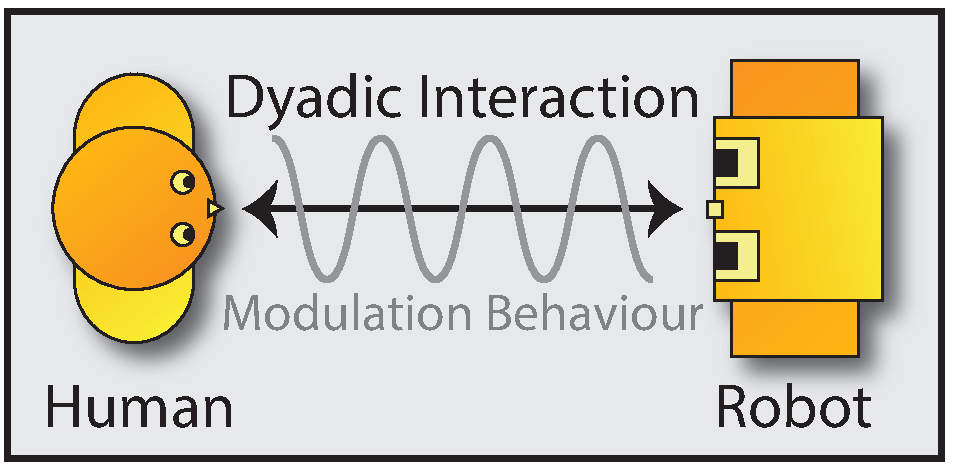
\includegraphics[width=0.48\textwidth]{images/ch4_DyadInteraction.pdf}
    \caption{Representation of the role of social cues in dyadic \acrshort{hri}. Social cues are used as modulation behaviour within the interaction.}
   \label{fig:ch4_dyadinteraction}
\end{figure}

Social behaviour plays a key role in dyadic interaction and on the outcome of communication within a dyad. The role of communication, or the social interaction within the dyad, in such a scenario is posited to be ``the mutual modification of two ongoing streams of behaviour of two persons'' \citep{beebe1992dyadic}. The behaviour of one party affects the behaviour of the other. In this view, social cues are used as part of the modulating behaviour in this process (Figure~\ref{fig:ch4_dyadinteraction}) and can therefore be utilised in many processes influencing education.

The joint modification of behaviour within the dyad gives rise to the need for regulation and alignment of behaviour in order to simultaneously transmit and receive information \citep{jaffe2001rhythms}. All parties engaging in a social interaction must continually adapt the social cues they are using in order to effectively construct the interaction \citep{green1985reading}; for example, verbal turn-taking must be regulated through the use of various social cues \citep{beebe1992dyadic}. Such regulation is important in learning interactions, indicating when it is appropriate for learners to ask questions, and when it is time for them to receive information; learning is more challenging without social cues or conventions to manage this turn-taking \citep{nicol2003social}. This simple coordination in interaction is vital and has been shown to influence cognition from infancy \citep{jaffe2001rhythms}. Even in unstructured interactions with robots, children appear to actively seek such turn-taking in interactions \citep{baxter2013emergence}.

These kinds of interaction phenomena are not catered for in \gls{nonverbalimm} measures. The evaluation in this chapter saw positive results, but the interaction between the robot and the humans was largely in one direction (the robot instructing the humans); the robot was not responsive to human social cues or behaviour. This is an area which needs further exploration in \acrshort{hri}: the question is when the interaction becomes more interactional than those presentational behaviours considered in the present study, do \gls{immediacy} principles hold, or are additional behaviours (such as turn-taking policies) required? In the absence of further evidence in such contexts, the application of the \gls{nonverbalimm} metric provides a suitable basis for initial investigation; this will be conducted in later chapters.

%%%%%%%%%%%%%%%%%%%%%%%%%%%%%%%%%%%%%%%%%%%%%%%%%%%%%%%%%%%%%%%%%%%%%%%%%%%%%%%%%%%
\subsection{Using Nonverbal Immediacy in HRI}\label{sec:disc-nvi}
Whilst the evaluation in this paper had positive results and confirmed (or partially confirmed) two of the three hypotheses, it should be made clear that there are limitations imposed by the study design which could inhibit how well these findings translate to other scenarios. The human condition was shown through a video, whereas the robots were physically present. This means that a comparison between the recall and \gls{nonverbalimm} scores from the human and the robot conditions could be influenced by embodiment, or social facilitation effects \citep{zajonc1965social}. It should be noted that in this study, there is no direct comparison between these conditions: comparisons are made within robot conditions, or from children and adults, but not between the human and robot conditions. 

Generally, the adult raters have high reliability levels, which reflects the behaviour seen in the literature. That this applies to ratings of robot behaviours indicates the applicability of the metric. Whereas the alpha statistic is lower for children, there are two points of note. Firstly, there remains a reasonable consistency for the ratings of the human condition -- this extends the literature by showing the ability of children (in addition to adults) to use the \gls{nonverbalimm} metric. Secondly, for both children and adults, there was agreement in the ordering of relative \gls{immediacy} levels between the conditions -- this indicates that the \gls{nonverbalimm} scale is sensitive enough for the present study, for both adults and children.

A number of caveats apply however that require further investigation. A high reliability score is found for the adults who saw a robot condition, but this is not so high for those who saw the human condition. This may be due to relatively low subject numbers when considering only the human condition (13 subjects), where inconsistency from one or two individual subjects could have a large impact on the alpha value. The reliability for the human is higher for children than for adults, suggesting the difference in subject numbers could be a factor. Alternatively, it could be a result of embodiment: the robot conditions were seen in person, whereas the human was shown on screen, which may have influenced the reporting of social behaviour on the questionnaire.

The Cronbach's alpha statistic for the children who saw a robot condition is considerably lower than that of the adults. This is not so surprising, given the complications highlighted in the literature of using questionnaires with children \citep{borgers2000children}. However, it may also be a product of limitations in robot social behaviour. Cronbach's alpha measures the internal consistency of questionnaire items. Whilst some inconsistency is likely due in part to child interpretations of negatively worded items \citep{borgers2004response}, there are some items within the questionnaire that the robot behaviour itself is probably not consistent in. For example, the questions related to smiling and frowning are opposites of each other in terms of calculating a value for the scale, but could both be answered as `never' performed, as the robot does not have moveable facial features. Such a response would provide maximum inconsistency between these items. This would not necessarily reflect the reliability of the questionnaire, but a limitation in the ability of the robot to implement all of the questionnaire items. The same argument could be made for the items concerning touch -- it could be considered that the robot never touches the observer, whilst also not `avoiding' touch, as the question is worded. Inclusion of these two behavioural elements (that were not possible in the evaluation here) in subsequent work exploring the use of \gls{nonverbalimm} for characterising robot social behaviour would likely yield higher reliability scores. For these reasons, it is argued that \gls{nonverbalimm} provides a suitable metric for use with children in this context, given that is has the sensitivity to detect differences between groups of children, and the advantages provided by the metric in providing a guideline set of cues for robot behaviour design (as described in Chapter~\ref{chap:background}).

The interaction was also over a very short period of time (approximately 4-5 minutes) and the measurement of learning was through recall. Although recall is a fundamental element of learning, it is very different from understanding or applying knowledge, or from the higher dimensions of learning as defined in the revised version of Bloom's taxonomy \citep{krathwohl2002revision}. Later chapters of this thesis will investigate the use of \gls{nonverbalimm} in slightly longer interactions, and in dyadic contexts, with generalised cognitive learning as a measure (Chapter~\ref{chap:nviexperiment}; \citealp{kennedy2015higher}).

%%%%%%%%%%%%%%%%%%%%%%%%%%%%%%%%%%%%%%%%%%%%%%%%%%%%%%%%%%%%%%%%%%%%%%%
\section{Summary} \label{sec:nvi-summary}
Nonverbal immediacy can be used to characterise social behaviour through observer-reports on the use of social cues, such as gaze and gesture. This chapter built on \acrshort{hhi} and \acrshort{hri} literature introduced in Chapter~\ref{chap:background} relating to these cues, which were implemented in an evaluation that compared an intended high \gls{nonverbalimm} and a low \gls{nonverbalimm} robot. A human condition was also included to link the work here to existing \gls{nonverbalimm} literature. Several hypotheses derived from the \gls{nonverbalimm} literature were confirmed. Both children and adults judge the \gls{immediacy} of humans and robots in a similar manner. The children's responses were more varied than the adults, but it was still possible to identify a significant difference in their perception of the social behaviour between the two robot conditions. Children also recalled more of the story when the robot used more \gls{nonverbalimm} behaviours, which demonstrates an effect predicted by the literature. While there are some limitations in the measure, it is proposed that \gls{nonverbalimm} could be used as an effective means of characterising robot social behaviour for human-robot interaction, for both adult and child subjects. Additionally, the findings here support the approach taken in Chapter~\ref{chap:method}: to use adults as post-hoc evaluators of robot \gls{nonverbalimm}, given that their perceptions reflect those of the children to some extent.